
\chapter{Introduction}\label{sec:introduction}

% SM QFT LHC CERN CMS
 One of the goals of modern society is
  to experimentally investigate particles and
  interactions, and 
  to achieve this goal, the governments from 
  nearly 100 %89
  different countries, states and territories are
  presently funding over 13,000 scientists, engineers 
  and technicians to build, operate, maintain 
  and analyze data from the
  Large Hadron Collider (LHC)
  at the European Center for Nuclear Research (CERN).
 This thesis presents analyses of data taken
  with the Compact Muon Solenoid (CMS) detector
  using proton-proton collisions provided by the LHC
  during its operation in 2012 and 2015.
 Using the 2012 data, a measurement
  of the production cross section for
  the standard model (SM) process
  \ppwbblnbb is performed,
  where $\ell$ is an electron or a muon.
 Using the 2015 data, the monophoton signature
  is examined in the context of the SM
  process \ppzgnng and as a search for
  evidence of dark matter (DM).

\section{The Standard Model}
\subsection{Standard Model Particles}
  The SM Lagrangian uses the
   Yang-Mills construction on the group
   $SU(3)\times SU(2)\times U(1)$.
  Strong interactions are described by the symmetry $SU(3)$ (color)
   which requires eight gauge bosons, known as gluons.
  Electroweak interactions are described by
   $SU(2)\times U(1)$ are moderated by the 
   massive $W^\pm$ and $Z$ bosons and the massless
   photon ($\gamma$).

%%%% TABLE Covariant derivatives and fermion couplings
\begin{table}[htb]\caption[Fermion couplings]
{
Fermions can exist in doublet and singlet configurations
 which are listed below along with the
 gauge fields the configuration interacts with,
 denoted by the symmetry the field respects. 
}
\label{tab:covarderivs}
\begin{center}
%\resizebox{\columnwidth}{!}{
\begin{tabular}{r|l|l|l}
%\begin{multirow}{2}{*}{ Name } & \begin{multirow}{2}{*}{ Covariant derivative } & \multicolumn{2}{c}{Interactions} \\
  \multicolumn{1}{c|}{}                       & \multicolumn{3}{c}{Interactions} \\
 %\cline{3-4}
  Fermion type & $SU(3)$ & $SU(2)$ & $U(1)$  \\
 \hline 
 \hline 
 All quarks  (doublet)      & Yes  & Yes & Yes \\
 All leptons (doublet)      & No   & Yes & Yes \\
 $u$-type quarks (singlet)  & Yes  & No  & Yes \\
 $d$-type quarks (singlet)  & Yes  & No  & Yes \\
 Charged leptons (singlet)  & No   & No  & Yes 
\end{tabular}
%}
\end{center}
\end{table}
%%%%%%%

 The matter and antimatter components
  are spin-$\sfrac{1}{2}$ fermions, which come
  in two families, known as leptons and quarks.
 Quarks and leptons come in three
  families, known as generations for the 
  quarks and flavors for the leptons.
 The leptons are colorless and therefore
  do not couple to gluons, but the 
  quarks do and additionally 
  come in three color varieties
  for each generation. % $(r,g,b) = $ (red, green, blue). 
 The singlet configurations contain only electrically charged
  fermions.

 All quarks and leptons can exist in $SU(2)$
  doublet configurations, and the different $I_3$ 
  values further break quarks and leptons into types.
 For quarks, there are $u$-type {$(u,c,t)=$ (up, charm, top)} which have charge $+\sfrac{2}{3}$,
  and there are $d$-type {$(d,s,b)=$ (down, strange, bottom)} which have charge $-\sfrac{1}{3}$.
 Leptons are either charged {$(e,\mu,\tau)=$ (electron, muon, tauon)}
  or neutral {$(\nu_e,\nu_\mu,\nu_\tau)=$ (electron-, mu-, tau-neutrino)},
  and all charged fermions are arranged such that mass
  increases with successive generations within a given type. 
 In units where $\hbar=c=1$, the top ($m_t=173 \;\GeV$)
  and bottom ($m_b=4 \;\GeV$) are the heaviest quarks
  of their respective types, with the bottom 
  weighing three orders of magnitude greater than 
  the lightest quark, up ($m_u=2 \;\MeV$).
 The mass separation for the charged leptons
  ($m_\tau=1.7 \;\GeV, m_e=0.5 \;\MeV$)
  also spans multiple orders of magnitude,
  but while the observations of neutrino oscillations
  indicate that neutrinos have mass, 
  only upper limits on the values they may have
  have been set on the order of \MeV. 

\subsection{Electroweak symmetry breaking}
 \label{sec:higgsmech}
 Fermions and gauge bosons
  acquire mass through the Brout-Englert-Higgs
  mechanism
  in which a  scalar field %obeying $SU(2)$ symmetry
  is introduced to the SM Lagrangian in the 
  doublet configuration.
 This generates mass for the Higgs boson ($m_H$)
  as well as for the
  $W^\pm$ and $Z$ bosons, while leaving the photon massless,
\begin{equation}\label{eq:bosons}
 M_Z = \frac{v}{2}\sqrt{g_1^2 + g_2^2}, \;\;\; M_W = \cos\theta_W M_Z\;\;\;,
\end{equation}  
  where the Weinberg angle, $\theta_W=\sfrac{g_1}{g_2}$,
  is the ratio between the $U(1)$ and $SU(2)$ coupling strengths,
  and $v\propto m_H$ is vacuum expectation value of the 
  Higgs field.
 The $\pm$ in $W^\pm$ aligns with the electric charge of
  the $W$ boson, % in units of $e$,
  and the $Z$ and $\gamma$ are both electrically neutral and orthogonal.

 The vector boson couplings to the fermions
  are then expressed as three types of currents.
 Electromagnetic interactions 
  involve couplings between the photon
  and charged particles,
  and any particle which interacts with the photon
  can also interact with the $Z$ boson. 
 The neutral current interactions have additional
  couplings to the lepton and quark doublets
  and charged current interactions
  are between the doublets and the $W$ bosons.
 Couplings to each of the bosons are scaled by
  a coupling factor which decides the relative
  strengths of the interactions.
 The coupling factors are related to the
  strengths of the unbroken
  $U(1)$ and $SU(2)$ couplings as
\begin{equation}
e   =  \frac{g_1 g_2}{\sqrt{g_1^2+g_2^2}},\;\;\;
g_Z =  \frac{e}{\cos \theta_W \sin \theta_W},\;\;\;
g_W =  \frac{e}{\sqrt{2} \sin \theta_W}
\end{equation}

 In addition to generating mass terms for the bosons,
  the Higgs field gives rise to fermion mass 
  via Yukawa couplings between the Higgs
  and fermion doublets.
 It is because the mass of the Higgs boson is tied
  to the masses of the gauge bosons and 
  charged fermions that the discovery of
  the Higgs boson in 2012
  was of such importance.
 The result was announced just a few months
  after I moved to Geneva
  to do research at CERN,
  and it provided the first measurement of
  a parameter in the SM that had been previously unknown,
  $m_H=125$ \GeV.

 To describe the scattering of fermions
  and gauge bosons in the SM,
  diagrams with the appropriate initial and final
  state particles are constructed from the 
  vertices illustrated in Figure~\ref{fig:smcouplings}.
 External lines correspond to real particles
  which are observed in the final state
  and are on-shell.
 Internal lines correspond to virtual
  particles that not observed in the 
  final state and therefore 
  may or may not be on-shell.
 A diagram is tree-level or leading order (LO) if it 
  uses the smallest number of vertices possible
  to depict an interaction having the
  correct initial and final states.

%%%%%%%%%%%%%
\begin{figure}[!htb]
 \center
 \caption[Illustrations of SM couplings]{
  The couplings for the SM gauge interactions.
 } 
 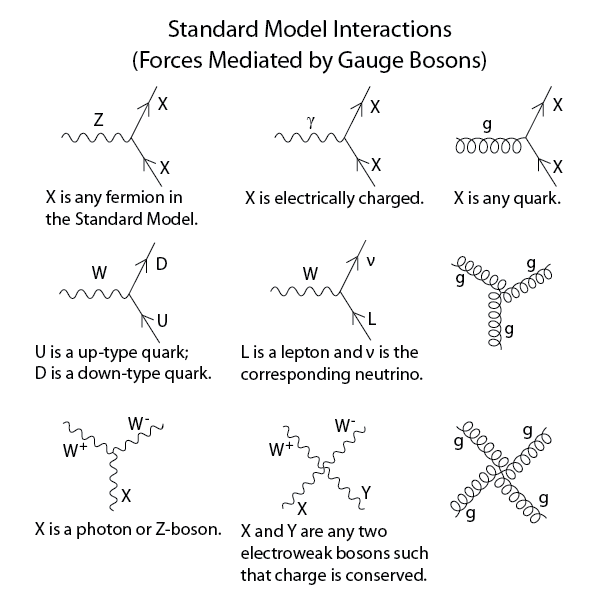
\includegraphics[width=0.6\textwidth]{/Users/rhombus/CMS/Thesis/thesis/pdfs/feyn/Standard_Model_Feynman_Diagram_Vertices.png}
    \label{fig:smcouplings}
\end{figure}
%%%%%%%%%%%%%

 Renormalization is necessary to account
  for corrections to the tree-level propagators
  and vertices which arise from contributions
  of virtual particles connecting to 
  form closed internal loops.
 The lowest order diagrams with
  one internal loop,
  are illustrated in Figure~\ref{fig:oneloopfeyn}.
 Because these diagrams contain the next fewest
  number of possible vertices above LO,
  they are termed next-to-LO (NLO).
 Renormalization is accomplished by introducing an energy scale,
  and assuming that the couplings are small compared 
  this this scale. 
 The coupling constants are therefore
  functions of energy 
  and are quoted at a particular renormalization scale,
  $\mu_R$.
 Renormalization works 
 Next-to-NLO 
 
 %% Determining if a theory is renormalizable
  % Srednicki 129, 18

 %% Consequences of running coupling constants ..

%%%%%%%%%%%%%
\begin{figure}[!tb]
 \center
 \caption[One-loop corrections to vertices and propagator]{
  Renormalization takes place via a modification
   of the coupling parameters $g_1,g_2,g_3$ to account
   for the contributions that loops of virtual
   particles make on the propagators and vertices.
  Below are diagrams keeping track of the
   flow of momentum for one-loop corrections to the 
   propagator and three and four point vertices.
 } 
 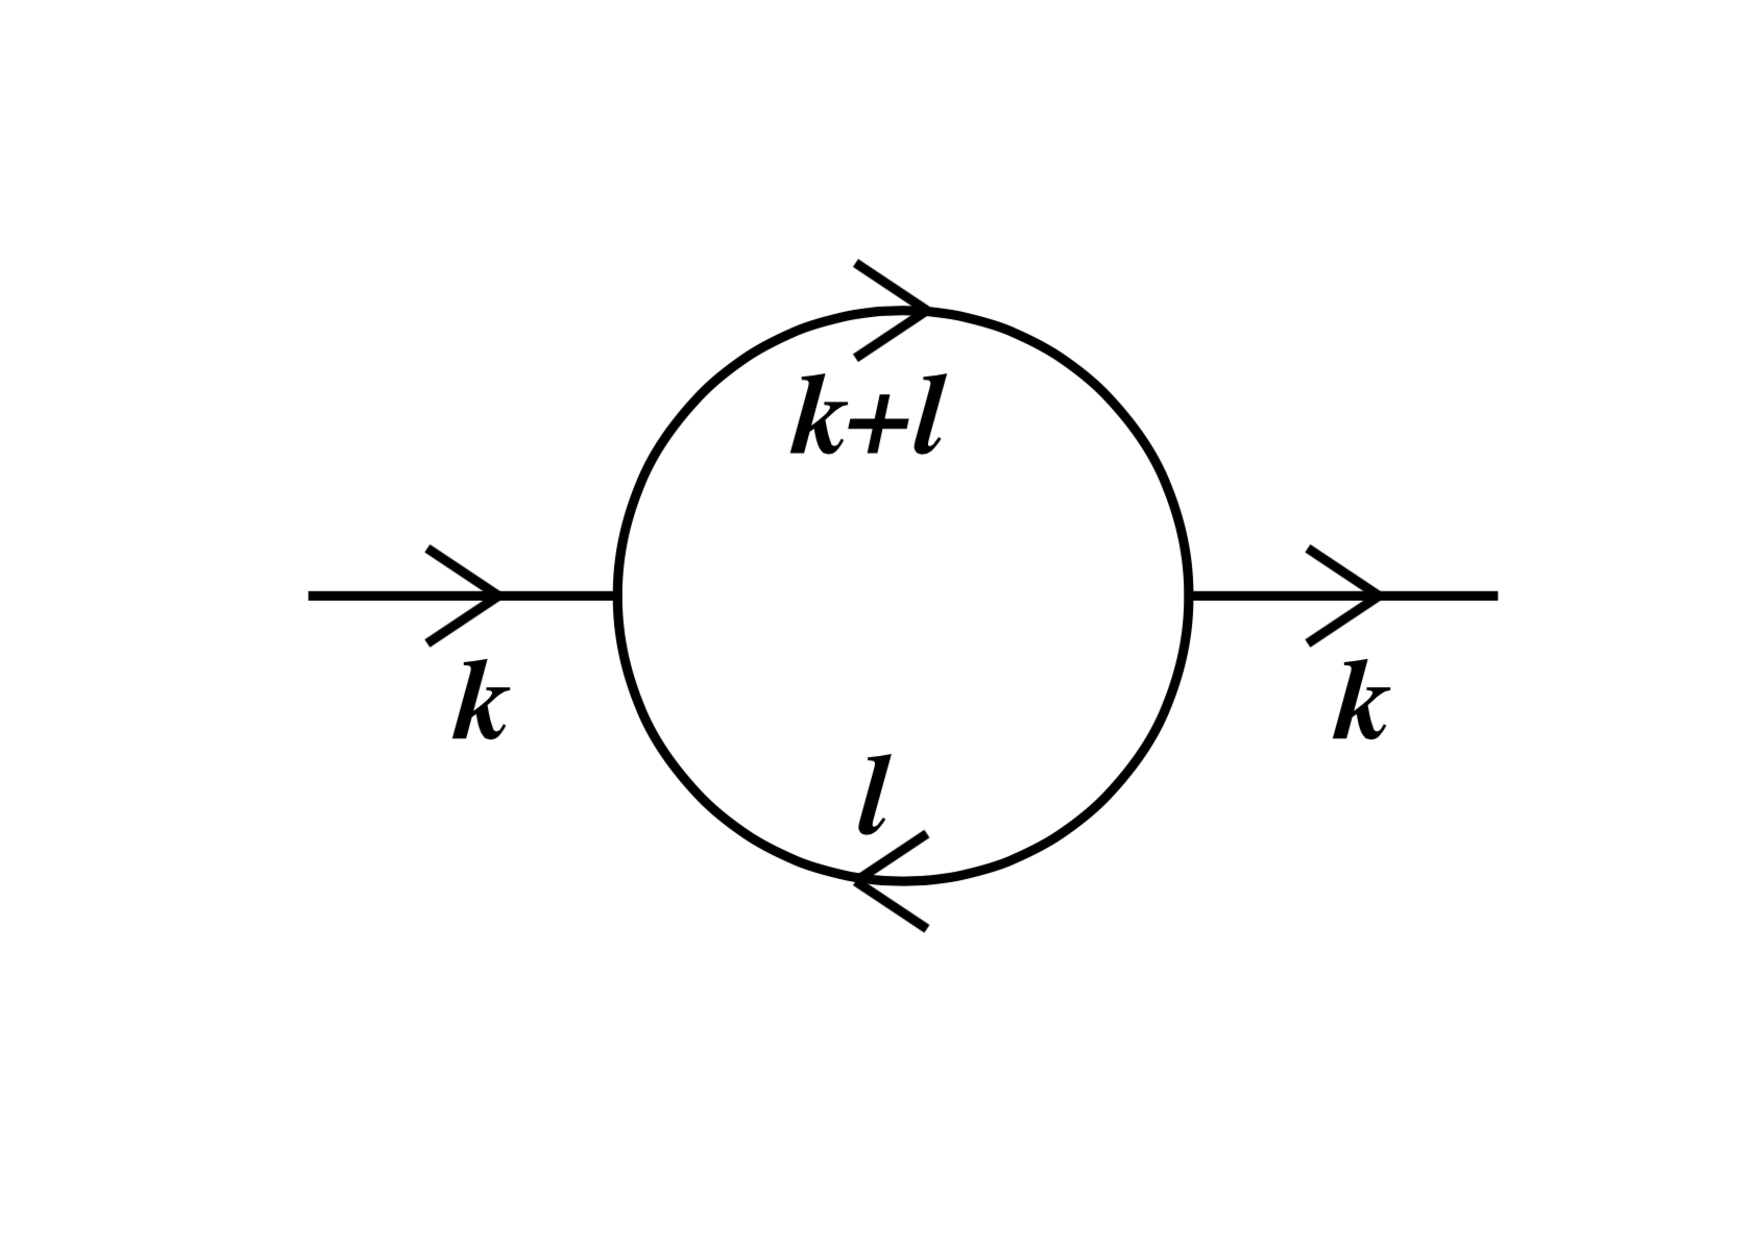
\includegraphics[width=0.3\textwidth]{/Users/rhombus/CMS/Thesis/thesis/pdfs/intro/loop_propagator.pdf}
 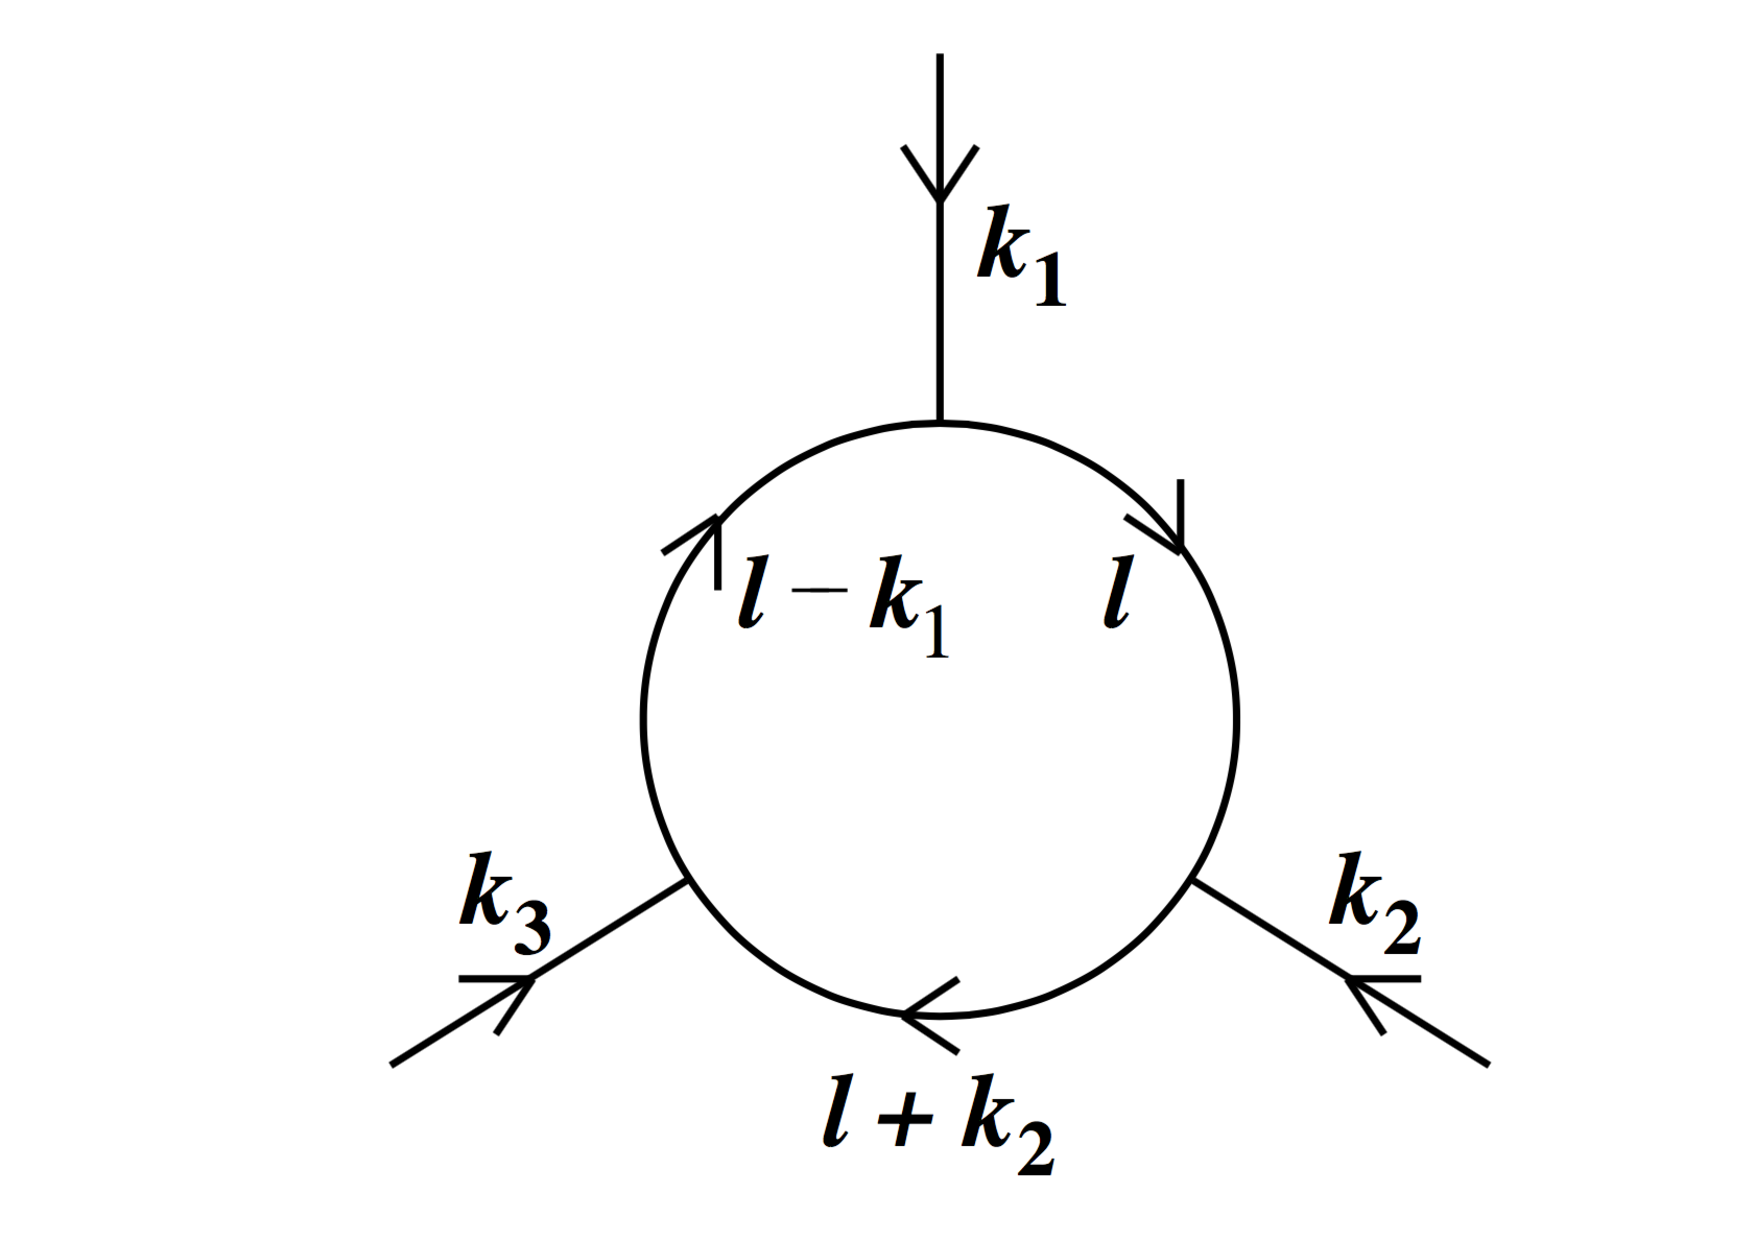
\includegraphics[width=0.3\textwidth]{/Users/rhombus/CMS/Thesis/thesis/pdfs/intro/loop_vertex.pdf}
 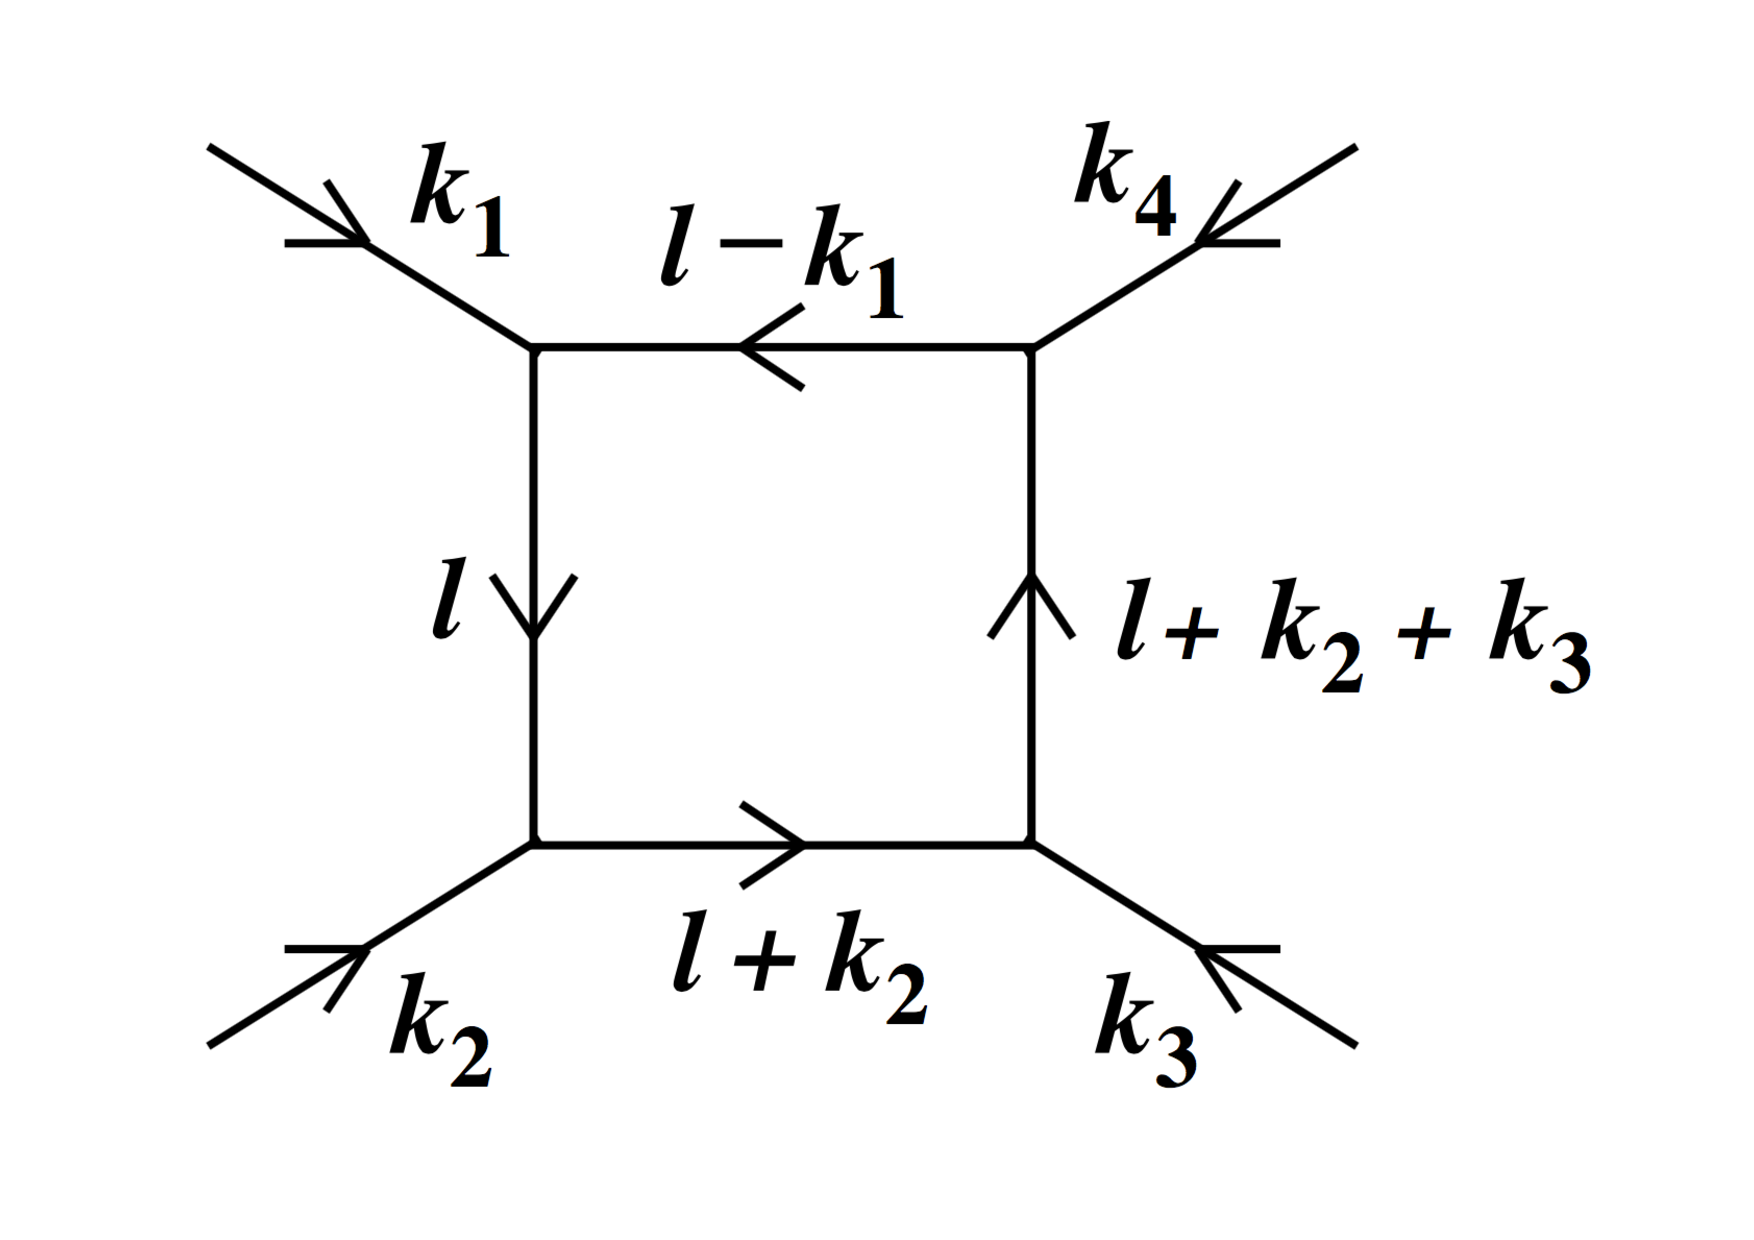
\includegraphics[width=0.3\textwidth]{/Users/rhombus/CMS/Thesis/thesis/pdfs/intro/loop_vertex4p.pdf}
    \label{fig:oneloopfeyn}
\end{figure}
%%%%%%%%%%%%%

%\subsection{Scattering amplitudes and cross sections}
\subsection{Cross sections and decay rates}

 Quantum mechanics dictates that 
  only predictions of probability are possible,
  and the final probability of observing
  a particular interaction
  is dependent on many variables, including
  the energies, types and angular momenta of the incoming
  and outgoing particles as well as
  the masses of the propagators
  and the orientation and efficiency of the detector.

 A quantity typically measured is therefore the 
  interaction cross section, $\sigma$,
  and for the scattering of two incoming 
  particles going to $n'$ particles, $2\rightarrow n'$,
  in the CM frame, the differential is
\begin{equation}\label{eq:dsigma}
 d\sigma = \frac{1}{4\abs{\mathbf{k}_1}_{\mathrm{CM}}}\abs{\mathcal{T}}^2 
  d\mathrm{LIPS}_{n'}(k_1 + k_2)
\end{equation}
  where the scattering matrix element, $\mathcal{T}$,
  is defined using Equation \ref{eq:lszformula}, as 
\begin{equation}\label{eq:matrixelement}
\langle f | i \rangle = (2\pi)^4\delta^4\left(\sum k_{\mathrm{in}}-\sum k_{\mathrm{out}}\right)
  i \mathcal{T}
\end{equation}
  and the Lorentz-invariant measure of the 
  phase space for the $n'$ outgoing particles is
\begin{equation}\label{eq:dlips}
 d\mathrm{LIPS}_{n'}(k) = (2\pi)^4 \delta^4
  \left(k - \sum_{j=1}^{n'}k'_i \right )
  \prod_{j=1}^{n'}dq_j'
\end{equation}
 with the Lorentz-invariant differential $dq$.

 The cross section is used to calculate the rate
  at which a process occurs, but is
  not the only relevant factor in determining
  the overall production rate.
 The production rate of a given final state
  is also dependent on the incoming
  rate of possible interactions and is 
  known as luminosity, \lumi.
 Luminosity has the units of inverse area per unit time
  and the total number of events produced
  is therefore proportional to \tlumi.
 In any real detector, final state particles
  are collected only within a finite
  solid angle and the number of particles
  scattered into a given solid angle, $\Omega$, is given by
\begin{equation}\label{eq:lumidef}
 \frac{dN}{d\Omega} = \lumi \frac{d\sigma}{d\Omega}\;\;\;.
\end{equation}


 %The rate at which a particular event occurs
 % is proportional to \lumi and the cross section 
 % of that interaction, so it is the
 % (time) integrated luminosity that determines 
 % the total number of events produced.

 It is also possible for particles to decay
  as $1\rightarrow n'$.
 Massive particles decay to lighter ones
  in both the fermion and boson sectors,
  with all massive bosons able to 
  spontaneously decay via the diagrams in
  Figure~\ref{fig:smcouplings}.
 Of the charged fermions, only the first
  generation is stable for each type, and
  neutrinos are not known to spontaneously
  decay, but oscillate between flavors
  while propagating in free space.
 Like the differential cross section,
  the differential decay rate is a function
  of the scattering amplitude and
  has integration measure $d\mathrm{LIPS}$, 
\begin{equation}\label{eq:diffdecayrate}
 d\Gamma = \frac{1}{2E}\abs{\mathcal{T}}^2d\mathrm{LIPS}_{n'}(k)\;\;\;.
\end{equation}

 The differential decay rate is 
  inversely proportional to the energy
  of the particle, $E=\sqrt{m^2 + p^2}$.
 This means that
  comparatively heavy particles will decay
  faster than comparatively light ones
  and that energetic particles
  will appear to live longer 
  for a stationary observer due to
  relativistic time dilation effects.
 The total decay rate of a given particle
  is found by summing the decay rates from
  each of the contributing processes,
  and the primary decay channels and rates
  for the fundamental particles
  are given in Table \ref{tab:lifetimes}.

 At CMS, the heaviest quark and the heaviest
  lepton both decay before reaching
  the detector volume.
 This makes $b$ quarks the heaviest
  fundamental particles which can be seen
  to decay inside the detector,
  and therefore an object of interest.
 Additionally, their heavy mass means that they
  couple strongly with the Higgs boson
  which still has many properties that
  are under investigation.
 The $W$ and $Z$ bosons are both so 
  massive that they decay before reaching
  the innermost layers of the detector
  and are often identified by their decay products
  pointing back to a common vertex.
 
%%%% Table SU(2) Representations
\begin{table}[tb]
\caption[Fundamental particle decay channels and rates]
{
 Below are listed the decay channels and 
  rates for each of the unstable
  fundamental particles.
 At CMS, with the detection apparatus
  located a finite distance away from the
  interaction vertex, particles such as the
  $W$, $Z$ and Higgs bosons,
  as well as the $t$ and $tau$, decay before
  reaching the first layer of the detector.
}
\label{tab:lifetimes}
\begin{center}
\resizebox{\columnwidth}{!}{
\begin{tabular}{r|l|l|l}
Particle & Primary decay modes(s) & Total rest-frame $d\Gamma$ & Typical decay location \\
\hline\hline
$W$ & $W\rightarrow \ell\nu$ & X & Before reaching CMS \\
$Z$ & $Z\rightarrow f\overline{f}$ (for $2M_f < M_Z$) & X & Before reaching CMS \\
$\tau$ & $\tau\rightarrow W \nu_\tau$ & X & Before reaching CMS \\
$\mu$  & $\mu\rightarrow W \nu_\mu$ & X & After leaving CMS \\
$t$    & $t\rightarrow W^+b$ & X & Before reaching CMS \\
$b$    & $b\rightarrow W^-c$ & X & Inside CMS \\
$c$    & $c\rightarrow W^+s$ & X & Inside CMS \\
$s$    & $s\rightarrow W^-u$ & X & Inside CMS
\end{tabular}
}
\end{center}
\end{table}
%%%%%%%
 

\subsection{QCD and Proton Structure}\label{sec:protonstructure}
 Feynman diagrams are used to %introduced in Section \ref{sec:PIandFD}
  describe interactions between fundamental particles,
  but at the LHC, collisions take place between
  protons, which are composite.

 One feature of the $SU(3)$ symmetry of the
  strong force is that gluons
  carry one unit of color and one unit of anticolor
  while the quarks carry one unit of color charge.
 This is what allows gluons to interact with each other
  as well as with quarks.
 That quark confinement is necessitated by the $SU(3)$
  structure has not been conclusively determined, 
  but observationally, a free gluon or quark has 
  never been observed.
 Instead, quarks appear as bound in colorless (singlet)
  combinations called hadrons
  which are further classified as mesons ($q\overline{q}$)
  or as baryons ($qqq$ or
  $\overline{q}\overline{q}\overline{q}$),
  and are held together by gluons.
 Evidently, the binding energy of the
  quarks has a form such that
  after a distance of roughly $10^{-15}$ meters,
  the energy
  stored in the gluon field is greater
  than the energy needed to create a
  quark-antiquark pair, bringing the pair
  into existence.
 This process of energetic quarks
  creating particles as they
  separate is called hadronization
  and is an important effect at the LHC.

 Protons are a type of baryon and
  at low energy, may combine with a single electron 
  to form a neutral hydrogen atom.
 At higher energies, the internal structure 
  of the proton becomes more evident,
  and it contains three valence quarks, $uud$, 
  which are constantly exchanging gluons.
 When probed at high enough energy, or equivalently,
  at short enough length scales, these 
  gluons can also each split into a $q\overline{q}$ pair 
  which typically reannihialate with each other.
 With gluons inside the proton splitting into quarks
  and coupling with other gluons,
  this forms a `sea' of quarks and gluons,
  and as protons are accelerated
  to energies of \GeV or \TeV as is the case at the
  LHC, the fraction of the momentum of the
  proton attributed to the gluons becomes higher 
  than that attributed to the valence quarks.

 A proton-proton collider was therefore a 
  sensible choice for the LHC. 
 The physics goals of the project are
  to measure quantities associated with a wide range SM 
  processes and to continue the search for 
  evidence of new physics.
 Quarks interact with all of the SM gauge bosons
  as well as with the Higgs boson
  and the proton contains the lightest
  quarks of each type
  in addition to the gluons and sea.
 Colliding proton beams thus allow for
  the interactions between many different
  initial particle configurations to be explored,
  and with the exception of the neutrinos which 
  interact only via the weak exchange of the $Z$
  boson and escape the detectors,
  all other fundamental SM particles have been
  directly  observed  at CERN. 

\section{Previous \wbb Measurements}

The production of
 \w bosons
 in association with $b$ jets has been 
 studied at a center-of-mass
 energy of 7 TeV using data samples with up
 to 5 \fbinv of integrated luminosity,
 by the ATLAS and CMS experiments \cite{Chatrchyan:2013uza,Aad:2013vka}, 
 as well as by the Collider Detector at Fermilab (CDF)
 and D0 Collaborations using \ppbar collisions
 provided by the Tevatron \cite{WbbTevD0,WbbTevCDF} at  
 Fermilab at $\sqrt{s}=1.96$ TeV. 
Neither of the experiments at the Tevatron
 directly examined a final state with 
 more than one $b$-tagged jet, 
 but both published results on the 
 process \ppbarwbjlnbj where $j$ signifies
 any jets.
The CDF Collaboration observed a cross section
 that was a factor of two higher than the best
 NLO prediction available at the time, and the 
 D0 Collaboration observed a cross section 
 that was $20\% - 40\%$ higher than 
 various NLO predictions.
The ATLAS Collaboration also examined a
 final state having only one $b$-tagged jet 
 in the process \ppwblnb.
They measured cross sections for 
 final states with
 exactly one jet 
 and exactly two jets, and 
 their observed cross section in the 
 one-jet channel was $70\%$ higher than the NLO prediction.
The agreement improved in the two-jet channel,
 where the observed cross section was $30\%$ higher
 than the NLO calculation predicts.

The first measurement of a final state
 having two identified $b$ jets
 and the products of a $W$ decay
 was made by the CMS Collaboration 
 at \s 7 \TeV
 in the process \ppwbbmnbb where 
 exclusively two jets were allowed,
 both of which $b$-tagged.
In this measurement, the 
 cross section was found to be  
 within $4\%$ of the NNLO prediction,
The analysis presented in this
 thesis extends the \ppwbbmnbb analysis
 to \s 8 \TeV and additionally incorporates $W$
 decays $W\rightarrow e\nu$,
 with the goal of providing a
 measurement of this process at higher
 energy than ever before and comparisons
 with the latest simulations and predictions.

\section{Dark Matter}

 \subsection{Experimental motivations}
  
 Albert Einstein's theory of general relativity, GR,
  has many experimental predictions which 
  run counter to human intuition.
 GR predicts that massive objects
  warp a four-dimensional spacetime and
  thus feel mutual attraction.
 This has as a consequence,
  the prediction that even massless objects
  such as photons will experience a 
  net deviation in their path
  near a massive object as a result of
  gravity and this effect was famously verified
  by Arthur Eddington
  through the observation of stars around the
  sun during a full solar eclipse. 
 More recently, the direct detection of
  gravitational waves by the LIGO
  Collaboration also aligns with the GR
  predictions of distorted spacetime
  around colliding black holes.
 The time distortion effects due to
  the varying strengths of Earth's gravitational
  field on the surface and at the GPS satellites,
  provide precise tests of the quantitative 
  predictions of GR.
 However, though these tests and others provide evidence that
  GR is an accurate theory of gravity,
  some basic predictions related to gravitational interactions 
  do not agree with observations,
  motivating the concept for DM.
  
 The first observational evidence for DM
  came from an analysis of the speeds of galaxies
  in the Coma cluster by Fritz Zwicky.
 The magnitude of the angular velocities of the
  galaxies was too great to be explained by the visible matter
  alone and DM is now believed to outweigh visible
  matter in a ratio of $5:1$ throughout the universe
  and $10:1$ throughout the Milky Way galaxy. 
  % http://map.gsfc.nasa.gov/universe/uni_matter.html

%[stability of spiral galaxies]
%
%[timescale of galactic formation / supergalactic structures]

  \subsection{Simplified theoretical models} 

  The defining features of DM are that
   it is massive and appears to interact
   on large scales only via the gravitational force.
  On the galactic and supergalactic scales,
   DM is distributed along similar structures
   as is visible matter, and it surrounds 
   visible matter in extended halos. 

  Because DM has not yet been observed, 
   the models of DM being considered in this thesis are
   simplified and based on minimal assumptions,
   the first being that DM is even capable of interacting
   with hadrons and is thus possible to produce
   at the LHC.
  While the visible sector of particles is diverse,
   the models used in this analysis
   consist of a single DM particle,
   $\chi$, which is assumed to be a fermion
   and may be different from $\overline{\chi}$.

  One way DM could couple to the SM is via the
   addition of a $U(1)$ symmetry that
   gives rise to a vector gauge mediator, $M$.
  If some quarks are also charged under
   $U(1)$, then DM may be produced in the
   $s$ channel as
   $f\overline{f}\rightarrow M\rightarrow\chi\overline{\chi}$.
  If $M$ conserves parity in $f\overline{f}\rightarrow M$,
   it is said to have a vector coupling,
   and if it violates parity, it is
   termed axial-vector.
  In these models, $M$ is assumed not
   to couple to leptons, but
   an effective field theory (EFT)
   model is also considered in this analysis
   which estimates a direct interaction
   between DM and photons. 
  This coupling is mediated by a vertex
   $\gamma\gamma\chi\overline{\chi}$.
   and allows for DM production via
   the channel
   $pp\rightarrow\gamma\rightarrow\gamma\chi\overline{\chi}$.


\subsection{Previous DM Searches}

A search for particle DM~\cite{Khachatryan:2014rwa}
  used $19.6$~\fbinv of $pp$ data collected in 2012 by the CMS Collaboration at
 \s 8 \TeV, but no evidence was found and a new upper limit
 for the DM cross section was set.
A similar search was performed by the ATLAS experiment~\cite{Aaboud:2016uro}
 using $3.2$~\fbinv of $pp$ collision data at \s 13 \TeV
 collected in 2015, but again  no evidence for new physics was found. 
This imposed limits on the possible masses DM particles
 and the mediator mass as $m_\chi > 150$ \GeV or
 $m_M > 710$ \GeV.
